\documentclass[12pt,a4paper]{article}
\usepackage[UTF8]{ctex}
\usepackage{amsmath,amssymb}
\usepackage{xcolor}
\usepackage{hyperref}
\usepackage{geometry}
\usepackage{graphicx}
\geometry{margin=2.5cm}

\title{Multiple Classical Registers / 多经典寄存器}
\author{QuoNic}
\date{}

\begin{document}
\maketitle

\begin{center}
\textbf{Language / 语言特性} | 难度：初级 | 预计时间：5 分钟
\end{center}

\tableofcontents
\newpage

\section{为什么需要？}

多经典寄存器用于在量子程序中存储多个测量结果。

\subsection{经典局限}
\begin{itemize}
  \item 单个经典寄存器只能存储一个测量结果
  \item 需要多个寄存器存储多个结果
\end{itemize}

\subsection{量子优势}
\begin{itemize}
  \item 多经典寄存器可以存储多个测量结果
  \item 支持复杂量子算法
  \item 是量子程序的基础组件
\end{itemize}

\subsection{实际应用}
\begin{itemize}
  \item 量子算法
  \item 量子纠错
  \item 量子通信
\end{itemize}

\section{快速上手}

\begin{verbatim}
from quonic import qgate, qshow
from quonic.gates import H

# 多经典寄存器
qgate(H, 0)
qgate(H, 1)
qshow()
\end{verbatim}

\textbf{预期输出}：
\begin{verbatim}
backend: native | shots: 1024
Result:
  |00>     256  ( 25.0%)
  |01>     256  ( 25.0%)
  |10>     256  ( 25.0%)
  |11>     256  ( 25.0%)
\end{verbatim}

\section{原理详解}

\subsection{电路图}

\begin{center}
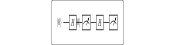
\includegraphics[width=0.6\textwidth]{../../images/creg_multi_circuit.svg}
\end{center}

\subsection{数学推导}

多经典寄存器：
\begin{equation}
\text{creg} = [c_0, c_1, \ldots, c_{n-1}]
\end{equation}

其中 $c_i$ 是经典比特。

\subsection{几何解释}

多经典寄存器在测量后存储多个经典比特。每个量子比特对应一个经典比特。

\section{代码详解}

\begin{verbatim}
from quonic import qgate, qshow
from quonic.gates import H

# 多量子比特测量
qgate(H, 0)
qgate(H, 1)

# qshow() 返回所有量子比特的测量结果
qshow()
\end{verbatim}

\section{进阶用法}

\subsection{场景 1：部分测量}

\begin{verbatim}
from quonic import qgate, qshow
from quonic.gates import H

# 部分测量
qgate(H, 0)
qgate(H, 1)
qshow(measure=[0])  # 只测量 q0
\end{verbatim}

\section{适用场景}

\subsection{量子算法}

多经典寄存器用于存储量子算法的多个测量结果。例如，Shor 算法需要存储多个量子比特的测量结果。

\subsection{量子纠错}

多经典寄存器用于存储量子纠错的伴随子测量结果。

\section{常见问题}

\subsection{多经典寄存器和单经典寄存器有什么区别？}

多经典寄存器可以存储多个测量结果，单经典寄存器只能存储一个。

\subsection{如何访问多经典寄存器？}

可以通过索引访问多经典寄存器。例如，\texttt{result[0]} 访问第一个经典比特。

\section{学习路径}

\subsection{前置知识}
\begin{itemize}
  \item 量子测量
  \item 经典寄存器
  \item 量子比特
\end{itemize}

\subsection{继续学习}
\begin{itemize}
  \item 量子算法
  \item 量子纠错
  \item 量子通信
\end{itemize}

\section{完整示例代码}

\subsection{示例 1：基本多经典寄存器}

\begin{verbatim}
from quonic import qgate, qshow
from quonic.gates import H

qgate(H, 0)
qgate(H, 1)
qshow()
\end{verbatim}

\section{下载}

\begin{itemize}
  \item [creg\_multi.py](https://github.com/ChrisLee0721/QuoNic/blob/main/examples/creg_multi/creg_multi.py)
\end{itemize}

\end{document}
